\documentclass[crop,tikz]{standalone}

\usepackage{amsmath}
\usepackage{xcolor}

\usetikzlibrary{arrows}
\usetikzlibrary{calc}
\usetikzlibrary{positioning}

\begin{document}
  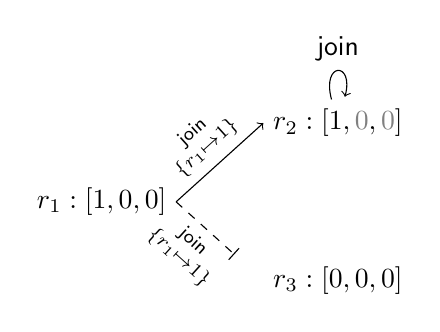
\begin{tikzpicture}
    \node (r1) at (0,0) {$r_1:[1,0,0]$};
    \node (r2) at (3, 1) {$r_2:[1, {\color{gray} 0},{\color{gray} 0}]$};
    \node (r3) at (3, -1) {$r_3:[0,0,0]$};

    \draw [->] (r1.east) -- node [midway, sloped, above] {$\substack{\textsf{join}\\\{ r_1 \mapsto 1 \}}$} (r2.west);

    \draw [-|,dashed] (r1.east) -- node [midway, sloped, below] {$\substack{\textsf{join}\\ \{ r_1 \mapsto 1 \}}$} ($(r1.east)!0.667!(r3.west)$);

    \draw [->] (r2) edge [loop above] node [above] {\textsf{join}} (r2);
  \end{tikzpicture}
\end{document}
